\documentclass[aspectratio=169,10pt]{beamer}
\usetheme{metropolis}
\usepackage{tikz}
\usetikzlibrary{calc,arrows.meta,angles,quotes}
\setbeamertemplate{navigation symbols}{}
\setbeamercolor{footline}{fg=white,bg=mDarkTeal}
\setbeamertemplate{footline}{%
\begin{beamercolorbox}[wd=\paperwidth,ht=3.2ex,dp=1.2ex]{footline}
\hspace{1.2em}\scriptsize Gajavada Sanjeevkumar\hfill
\scriptsize Engineering Curves: Epicycloid\hfill
\scriptsize
\Acrobatmenu{FirstPage}{\fbox{\(\blacktriangleleft\!\blacktriangleleft\)}}\,\Acrobatmenu{PrevPage}{\fbox{\(\blacktriangleleft\)}}\,\Acrobatmenu{NextPage}{\fbox{\(\blacktriangleright\)}}\,\Acrobatmenu{LastPage}{\fbox{\(\blacktriangleright\!\blacktriangleright\)}}\quad
\insertframenumber\hspace{1.2em}
\end{beamercolorbox}}
\title[Engineering Curves: Epicycloid]{Engineering Curves: Construction of Epicycloid}
\subtitle{Rolling Circle Method with Tangent \& Normal}
\author{Gajavada Sanjeevkumar}
\date{\today}

% =========================================================
% FULL-SLIDE WATERMARK
% =========================================================
\setbeamertemplate{background}{%
  \begin{tikzpicture}[remember picture,overlay]
    \node[
      rotate=32,
      text=black!12,
      font=\fontsize{30}{36}\selectfont,
      align=center,
      inner sep=0pt
    ] at (current page.center) {Gajavada Sanjeevkumar};
  \end{tikzpicture}%
}
\tikzset{extension line/.style={thin,densely dotted,black!60},directing line/.style={thick,blue!80!black},generating line/.style={thick,green!55!black},centre line/.style={thin,dash pattern=on 8pt off 2pt on 1.5pt off 2pt,black!65},construction line/.style={thin,cyan!75!black},division line/.style={thin,brown!80!black},arc line/.style={thin,purple!70!black},main curve/.style={thick,blue!85!black},normal line/.style={thick,orange!85!black},tangent line/.style={thick,magenta!80!black},contact line/.style={thin,black!65},dimension line/.style={thin,<->,>=Stealth,black!75}}
\newcommand{\Legend}[1]{\node[draw=gray!35,fill=white,rounded corners=2pt,inner sep=3pt,anchor=north east,align=left,font=\scriptsize,text width=31mm] at (84,84){#1};}
\newcommand{\Base}{\coordinate(O)at(0,0);\coordinate(A)at(150:45);\coordinate(B)at(30:45);\coordinate(Czero)at(150:60);\draw[thin](O)--(A);\draw[thin](O)--(B);\draw[extension line](A)--(150:82);\draw[extension line](B)--(30:82);\draw[directing line](A)arc(150:30:45);\fill(O)circle(.7pt)node[below]{$O$};\fill(A)circle(.55pt)node[above left]{$A$};\fill(B)circle(.55pt)node[above right]{$B$};}
\newcommand{\OADim}{\draw[dimension line]($(O)+(240:6)$)--($(A)+(240:6)$)node[midway,sloped,above,fill=white,inner sep=1pt,font=\scriptsize]{$45\ \mathrm{mm}$};\draw[thin,black!55]($(O)+(240:1)$)--($(O)+(240:8)$);\draw[thin,black!55]($(A)+(240:1)$)--($(A)+(240:8)$);}
\newcommand{\ACDim}{\draw[dimension line]($(A)+(60:4)$)--($(Czero)+(60:4)$)node[midway,sloped,above,fill=white,inner sep=1pt,font=\scriptsize]{$15\ \mathrm{mm}$};\draw[thin,black!55]($(A)+(60:1)$)--($(A)+(60:6)$);\draw[thin,black!55]($(Czero)+(60:1)$)--($(Czero)+(60:6)$);}
\newcommand{\DrawCzero}{\draw[centre line](O)--(Czero);\fill[black](Czero)circle(.55pt)node[above left]{$C_0$};}
\newcommand{\GenCircle}{\draw[generating line](Czero)circle(15);}
\newcommand{\GenPt}[1]{\coordinate(G#1)at($(Czero)+({330+30*(#1)}:15)$);}
\newcommand{\GenRad}[1]{\draw[construction line](Czero)--(G#1);}
\newcommand{\GenLab}[1]{\node[font=\tiny,green!45!black]at($(Czero)+({330+30*(#1)}:18.5)$){$#1$};}
\newcommand{\AllGen}{\foreach\k in{0,...,12}{\GenPt{\k}}}
\newcommand{\AllGenRad}{\foreach\k in{0,...,11}{\GenRad{\k}}}
\newcommand{\AllGenLab}{\node[font=\tiny,green!45!black,below right,inner sep=.5pt]at($(G0)+(330:2)$){$0,12$};\foreach\k in{1,...,11}{\GenLab{\k}};}
\newcommand{\ConArc}[1]{\pgfmathsetmacro{\aa}{atan2(60*sin(150-10*(#1))+15*sin(330+30*(#1)),60*cos(150-10*(#1))+15*cos(330+30*(#1)))}\pgfmathsetmacro{\rr}{sqrt((60*cos(150-10*(#1))+15*cos(330+30*(#1)))^2+(60*sin(150-10*(#1))+15*sin(330+30*(#1)))^2)}\draw[arc line](\aa:\rr)arc(\aa:{180-\aa}:\rr);}
\newcommand{\ConArcFixed}[2]{\pgfmathsetmacro{\bb}{300-(#1)}\draw[arc line](#1:#2)arc(#1:\bb:#2);}
\newcommand{\ConArcZero}{\draw[arc line](150:45)arc(150:30:45);}
\newcommand{\ConArcOne}{\draw[arc line](159.06468:47.60414)arc(159.06468:30:47.60414);}
\newcommand{\ConArcTwo}{\draw[arc line](163.89789:54.08327)arc(163.89789:30:54.08327);}
\newcommand{\ConArcThree}{\draw[arc line](164.03624:61.84658)arc(164.03624:30:61.84658);}
\newcommand{\ConArcFour}{\draw[arc line](160.89339:68.73864)arc(160.89339:30:68.73864);}
\newcommand{\ConArcFive}{\draw[arc line](155.86674:73.37469)arc(155.86674:30:73.37469);}
\newcommand{\ConArcSix}{\draw[arc line](150:75)arc(150:30:75);}
\newcommand{\CentreArc}{\draw[centre line](150:60)arc(150:30:60);}
\newcommand{\DivLine}[1]{\draw[division line](O)--({150-10*(#1)}:75);}
\newcommand{\DivLabel}[1]{\node[font=\tiny,orange!90!black,inner sep=0.5pt]at({150-10*(#1)}:43.2){$#1^\prime$};}
\newcommand{\CenterPt}[1]{\coordinate(C#1)at({150-10*(#1)}:60);\node[fill=black,circle,minimum size=2.6pt,inner sep=0pt,outer sep=0pt,transform shape=false]at(C#1){};\node[font=\tiny,above right,inner sep=.5pt]at(C#1){$C_{#1}$};}
\newcommand{\AllDiv}{\foreach\k in{0,...,12}{\DivLine{\k}}}
\newcommand{\AllLabels}{\foreach\k in{0,...,12}{\DivLabel{\k}}}
\newcommand{\AllCenters}{\foreach\k in{0,...,12}{\CenterPt{\k}}}
\newcommand{\AllPCoords}{\foreach\k in{0,...,12}{\coordinate(P\k)at({60*cos(150-10*(\k))+15*cos(330-40*(\k))},{60*sin(150-10*(\k))+15*sin(330-40*(\k))});}}
\newcommand{\CutArc}[1]{\pgfmathsetmacro{\qa}{330-40*(#1)}\draw[construction line,very thin](C#1)+({\qa-12}:15)arc({\qa-12}:{\qa+12}:15);}
\newcommand{\Pmark}[1]{\node[fill=black,circle,minimum size=2.6pt,inner sep=0pt,outer sep=0pt,transform shape=false]at(P#1){};\node[font=\tiny,blue!85!black,above right,inner sep=.5pt]at(P#1){$P_{#1}$};}
\newcommand{\AllCut}{\AllPCoords\foreach\k in{0,...,12}{\CutArc{\k}\Pmark{\k}}}
\newcommand{\Curve}{\AllPCoords\draw[main curve]plot[smooth]coordinates{(P0)(P1)(P2)(P3)(P4)(P5)(P6)(P7)(P8)(P9)(P10)(P11)(P12)};}
\newcommand{\SelectedGeometry}{\coordinate(Psel)at(-10.3596467,73.8670712);\coordinate(Cp)at(95:60);\coordinate(M)at(95:45);\coordinate(T1)at(14.0477535,79.2780615);\coordinate(T2)at(-34.7670469,68.4560808);\coordinate(NNleft)at(-0.7031893,30.3096065);\coordinate(NNright)at(-13.5784658,88.3862261);}
\newcommand{\PGeometry}{\node[fill=black,circle,minimum size=3.0pt,inner sep=0pt,outer sep=0pt,transform shape=false]at(Psel){};\node[font=\scriptsize,blue!80!black,above right,inner sep=.5pt]at(Psel){$P$};}
\newcommand{\PtoCpArc}{\draw[construction line,very thin](Psel)+(-82:15)arc(-82:-58:15);\draw[construction line](Psel)--(Cp);\node[fill=black,circle,minimum size=3.0pt,inner sep=0pt,outer sep=0pt,transform shape=false]at(Cp){};\node[font=\scriptsize,above right,inner sep=.5pt]at(Cp){$C_p$};\draw[dimension line]($(Psel)+(20:5)$)--($(Cp)+(20:5)$)node[midway,fill=white,inner sep=1pt,font=\scriptsize]{$15\ \mathrm{mm}$};}
\newcommand{\NormalAndTangent}{\draw[normal line,line width=1.2pt](NNleft)--(NNright);\node[font=\scriptsize,orange!85!black,above right,xshift=2pt]at(NNright){$N\prime$};\node[font=\scriptsize,orange!85!black,below left,xshift=-2pt]at(NNleft){$N$};\draw[tangent line,line width=1.2pt](T2)--(T1);\node[font=\scriptsize,magenta!80!black,below left,xshift=-2pt]at(T2){$T$};\node[font=\scriptsize,magenta!80!black,above right,xshift=2pt]at(T1){$T\prime$};}
\newcommand{\BaseCommon}{\Base\DrawCzero\GenCircle}
\newcommand{\GenFull}{\AllGen\AllGenRad\node[font=\tiny,green!45!black,below right,inner sep=.5pt]at($(G0)+(330:2)$){$0,12$};\foreach\j in{1,...,11}{\GenLab{\j}}}
\newcommand{\ConFull}{\ConArcZero\ConArcOne\ConArcTwo\ConArcThree\ConArcFour\ConArcFive\ConArcSix}
\newcommand{\DivFull}{\AllDiv\AllLabels\AllCenters}
\newcommand{\FinalConstruction}{\BaseCommon\GenFull\ConFull\CentreArc\DivFull\AllCut\Curve\foreach\k in{0,...,12}{\Pmark{\k}}}
\begin{document}
\begin{frame}[plain]\titlepage\end{frame}
\begin{frame}{Problem Statement}
\begin{block}{Problem}
\vspace{0.35em}
A generating circle of diameter $30$ mm rolls externally without slipping on a directing circle of diameter $90$ mm. Construct one complete epicycloid arch corresponding to $\angle AOB=120^\circ$, divide the arch into 12 equal angular parts, and retain every construction element in all subsequent views.
\vspace{0.35em}
\end{block}
\end{frame}
\begin{frame}{Given Data and Calculations}
\begin{columns}[T,onlytextwidth]
\column{0.49\textwidth}
\textbf{Given data}
\begin{align*}
\text{Diameter of directing circle} &=90\text{ mm},\\
R&=45\text{ mm},\\
\text{Diameter of generating circle} &=30\text{ mm},\\
r&=15\text{ mm},\\
\angle AOB&=120^\circ,\\
\text{Let number of divisions}&=12.
\end{align*}
\vspace{-0.4em}
\textbf{Calculations}
\begin{align*}
OC_0&=R+r=45+15=60\text{ mm},\\
AC_0&=r=15\text{ mm},\\
\Delta\theta&=\frac{120^\circ}{12}=10^\circ.
\end{align*}
\column{0.49\textwidth}
\textbf{Generating-circle division}
\begin{align*}
\text{Division angle}&=\frac{360^\circ}{12}=30^\circ.
\end{align*}
\vspace{0.3em}
\textbf{Rolling relation}
\begin{align*}
\text{Each }10^\circ\text{ centre step}&\leftrightarrow 30^\circ\text{ generating-circle step}.
\end{align*}
\end{columns}
\end{frame}
\begin{frame}{Step 1: Draw $OA$}\centering\begin{tikzpicture}[scale=.075,>=stealth]\coordinate(O)at(0,0);\coordinate(A)at(150:45);\draw[thin](O)--(A);\OADim\fill(O)circle(.7pt)node[below]{$O$};\fill(A)circle(.55pt)node[above left]{$A$};\Legend{$OA=45$ mm.}\end{tikzpicture}\end{frame}
\begin{frame}{Step 2: Extend $OA$}\centering\begin{tikzpicture}[scale=.075,>=stealth]\coordinate(O)at(0,0);\coordinate(A)at(150:45);\draw[thin](O)--(A);\draw[extension line](A)--(150:82);\fill(O)circle(.7pt)node[below]{$O$};\fill(A)circle(.55pt)node[above left]{$A$};\Legend{Extend $OA$.}\end{tikzpicture}\end{frame}
\begin{frame}{Step 3: Draw $OB$ at $120^\circ$}\centering\begin{tikzpicture}[scale=.075,>=stealth]\coordinate(O)at(0,0);\coordinate(A)at(150:45);\coordinate(B)at(30:45);\draw[thin](O)--(A);\draw[extension line](A)--(150:82);\draw[thin](O)--(B);\draw[thin] (150:15) arc (150:30:15);\node[font=\scriptsize]at(90:20){$120^\circ$};\fill(O)circle(.7pt)node[below]{$O$};\fill(A)circle(.55pt)node[above left]{$A$};\fill(B)circle(.55pt)node[above right]{$B$};\Legend{$\angle AOB=120^\circ$.}\end{tikzpicture}\end{frame}
\begin{frame}{Step 4: Extend $OB$}\centering\begin{tikzpicture}[scale=.075,>=stealth]\coordinate(O)at(0,0);\coordinate(A)at(150:45);\coordinate(B)at(30:45);\draw[thin](O)--(A);\draw[extension line](A)--(150:82);\draw[thin](O)--(B);\draw[extension line](B)--(30:82);\fill(O)circle(.7pt)node[below]{$O$};\fill(A)circle(.55pt)node[above left]{$A$};\fill(B)circle(.55pt)node[above right]{$B$};\Legend{Extend $OB$.}\end{tikzpicture}\end{frame}
\begin{frame}{Step 5: Draw the directing arc $AB$}\centering\begin{tikzpicture}[scale=.075,>=stealth]\Base\Legend{Blue arc $AB$: directing circle.}\end{tikzpicture}\end{frame}
\begin{frame}{Step 6: Locate $C_0$ and the generating circle}\centering\begin{tikzpicture}[scale=.075,>=stealth]\Base\DrawCzero\ACDim\GenCircle\Legend{$AC_0=15$ mm.\\Green: generating circle.}\end{tikzpicture}\end{frame}
\newcommand{\GenDivisionFrame}[1]{\begin{frame}{Step 7: Divide the generating circle into 12 equal parts}\centering\begin{tikzpicture}[scale=.075,>=stealth]\Base\DrawCzero\GenCircle\foreach\j in{0,...,#1}{\GenPt{\j}\ifnum\j>0\GenRad{\j}\fi}\ifnum#1<12\node[font=\tiny,green!45!black,below right,inner sep=.5pt]at($(G0)+(330:2)$){$0$};\foreach\j in{1,...,#1}{\GenLab{\j}}\else\node[font=\tiny,green!45!black,below right,inner sep=.5pt]at($(G0)+(330:2)$){$0,12$};\foreach\j in{1,...,11}{\GenLab{\j}}\fi\Legend{Green: generating circle.\\$30^\circ$ divisions.}\end{tikzpicture}\end{frame}}
\GenDivisionFrame{1}\GenDivisionFrame{2}\GenDivisionFrame{3}\GenDivisionFrame{4}\GenDivisionFrame{5}\GenDivisionFrame{6}\GenDivisionFrame{7}\GenDivisionFrame{8}\GenDivisionFrame{9}\GenDivisionFrame{10}\GenDivisionFrame{11}\GenDivisionFrame{12}
\begin{frame}{Step 8: Complete the generating-circle divisions}\centering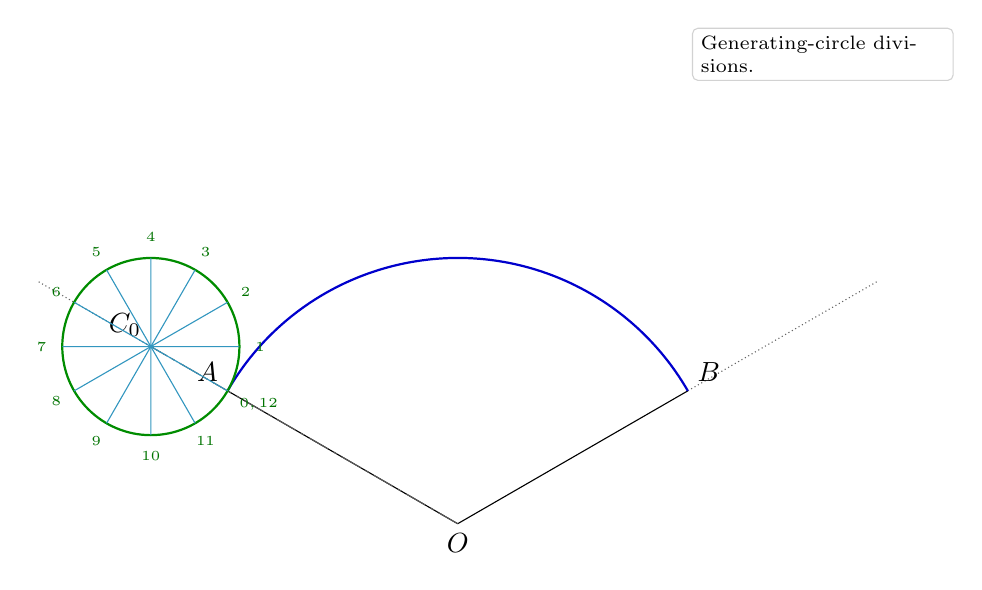
\begin{tikzpicture}[scale=.075,>=stealth]\Base\DrawCzero\GenCircle\GenFull\Legend{Generating-circle divisions.}\end{tikzpicture}\end{frame}
\newcommand{\ConFrame}[2]{\begin{frame}{Step 9: Draw concentric construction arcs}\centering\begin{tikzpicture}[scale=.075,>=stealth]\Base\DrawCzero\GenCircle\GenFull#2\Legend{Concentric construction arc.}\end{tikzpicture}\end{frame}}
\ConFrame{0}{\ConArcZero}
\ConFrame{1}{\ConArcZero\ConArcOne}
\ConFrame{2}{\ConArcZero\ConArcOne\ConArcTwo}
\ConFrame{3}{\ConArcZero\ConArcOne\ConArcTwo\ConArcThree}
\ConFrame{4}{\ConArcZero\ConArcOne\ConArcTwo\ConArcThree\ConArcFour}
\ConFrame{5}{\ConArcZero\ConArcOne\ConArcTwo\ConArcThree\ConArcFour\ConArcFive}
\ConFrame{6}{\ConArcZero\ConArcOne\ConArcTwo\ConArcThree\ConArcFour\ConArcFive\ConArcSix}
\begin{frame}{Step 10: Draw the centre arc through $C_0$}\centering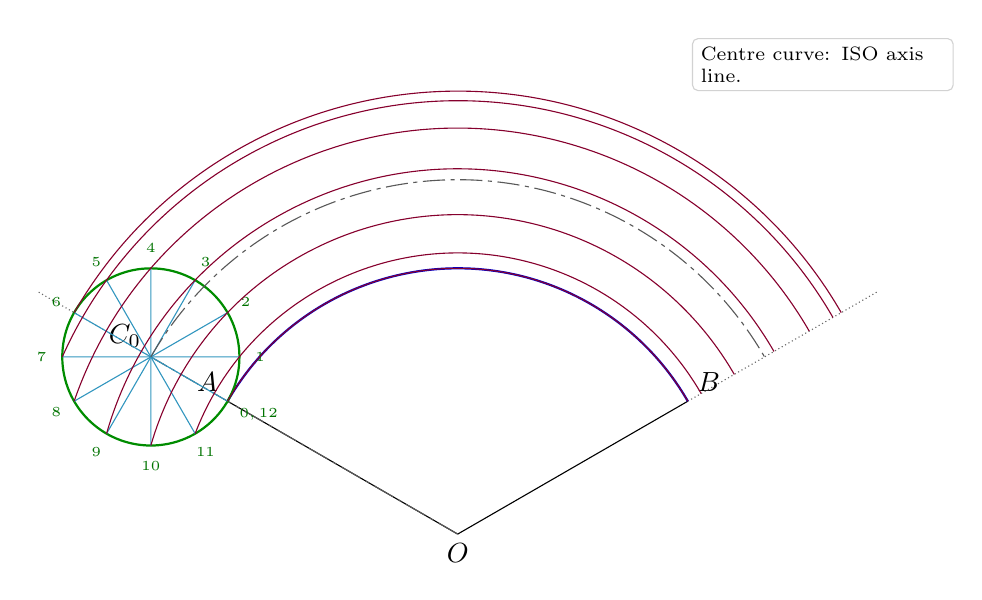
\begin{tikzpicture}[scale=.075,>=stealth]\Base\DrawCzero\GenCircle\GenFull\ConFull\CentreArc\Legend{Centre curve: ISO axis line.}\end{tikzpicture}\end{frame}
\newcommand{\AngleFrame}[1]{\begin{frame}{Step 11: Divide $\angle AOB$ into 12 equal parts}\centering\begin{tikzpicture}[scale=.075,>=stealth]\Base\DrawCzero\GenCircle\GenFull\ConFull\CentreArc\foreach\j in{0,...,#1}{\DivLine{\j}\DivLabel{\j}\CenterPt{\j}}\Legend{$10^\circ$ divisions.}\end{tikzpicture}\end{frame}}
\AngleFrame{0}\AngleFrame{1}\AngleFrame{2}\AngleFrame{3}\AngleFrame{4}\AngleFrame{5}\AngleFrame{6}\AngleFrame{7}\AngleFrame{8}\AngleFrame{9}\AngleFrame{10}\AngleFrame{11}\AngleFrame{12}
\begin{frame}{Step 12: Complete the angular divisions and points}\centering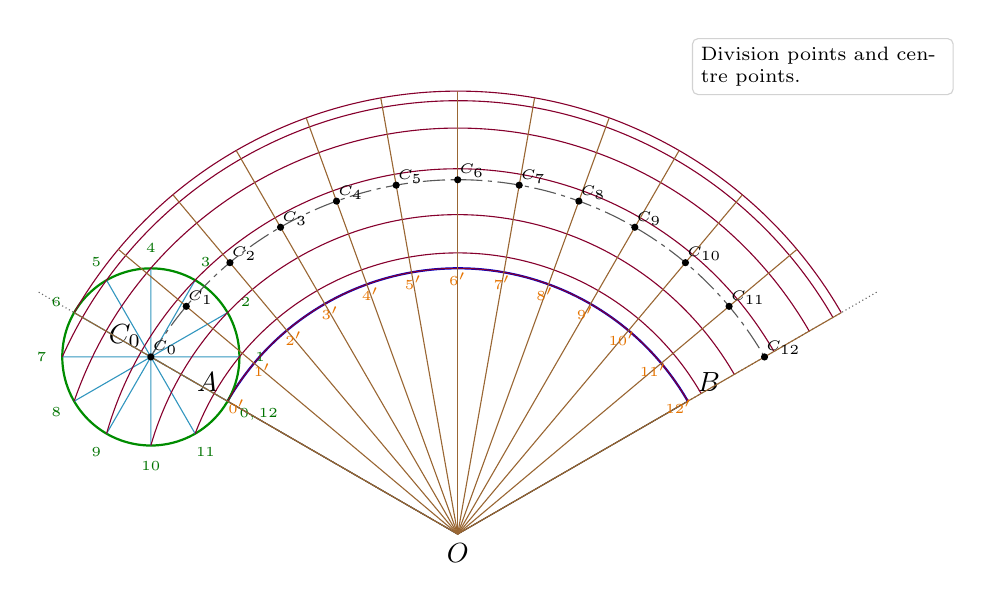
\begin{tikzpicture}[scale=.075,>=stealth]\Base\DrawCzero\GenCircle\GenFull\ConFull\CentreArc\DivFull\Legend{Division points and centre points.}\end{tikzpicture}\end{frame}
\newcommand{\CutFrame}[1]{\begin{frame}{Step 13: Draw the small cutting arc and locate $P_i$}\centering\begin{tikzpicture}[scale=.075,>=stealth]\Base\DrawCzero\GenCircle\GenFull\ConFull\CentreArc\DivFull\AllPCoords\foreach\j in{0,...,#1}{\CutArc{\j}\Pmark{\j}}\Legend{Cyan arc: radius $15$ mm.}\end{tikzpicture}\end{frame}}
\CutFrame{0}\CutFrame{1}\CutFrame{2}\CutFrame{3}\CutFrame{4}\CutFrame{5}\CutFrame{6}\CutFrame{7}\CutFrame{8}\CutFrame{9}\CutFrame{10}\CutFrame{11}\CutFrame{12}
\begin{frame}{Step 14: Draw the epicycloid}\centering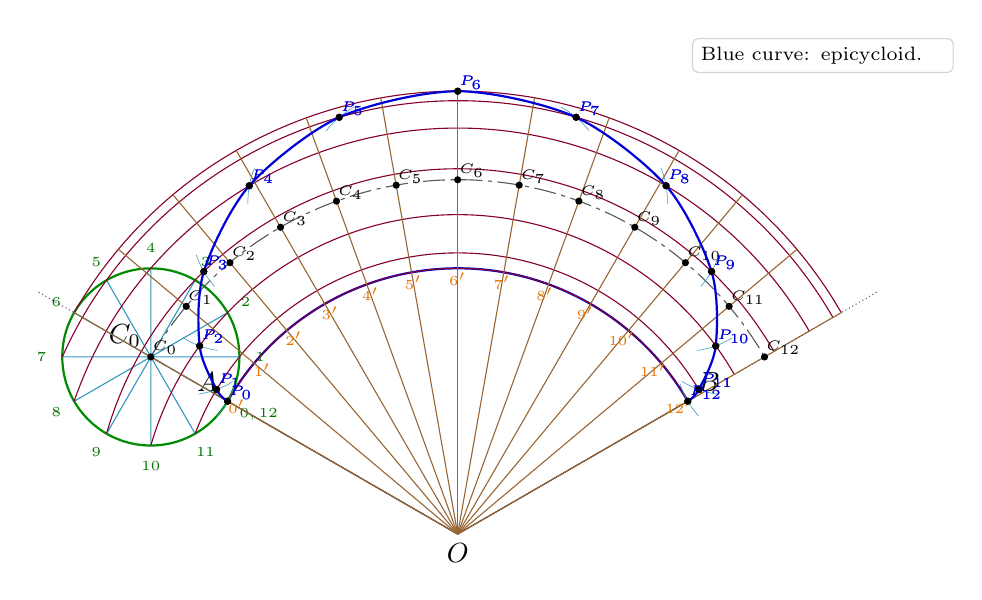
\begin{tikzpicture}[scale=.075,>=stealth]\FinalConstruction\Legend{Blue curve: epicycloid.}\end{tikzpicture}\end{frame}
\begin{frame}{Step 15: Select a point $P$ on the epicycloid}\centering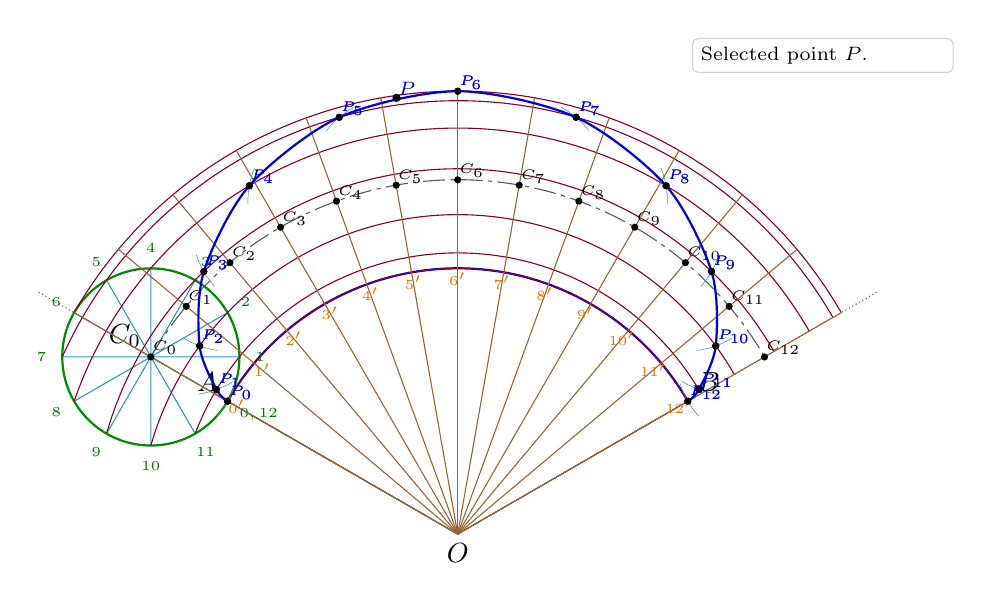
\begin{tikzpicture}[scale=.075,>=stealth]\FinalConstruction\SelectedGeometry\PGeometry\Legend{Selected point $P$.}\end{tikzpicture}\end{frame}
\begin{frame}{Step 16: Draw the $15$ mm arc from $P$ to the centre curve}\centering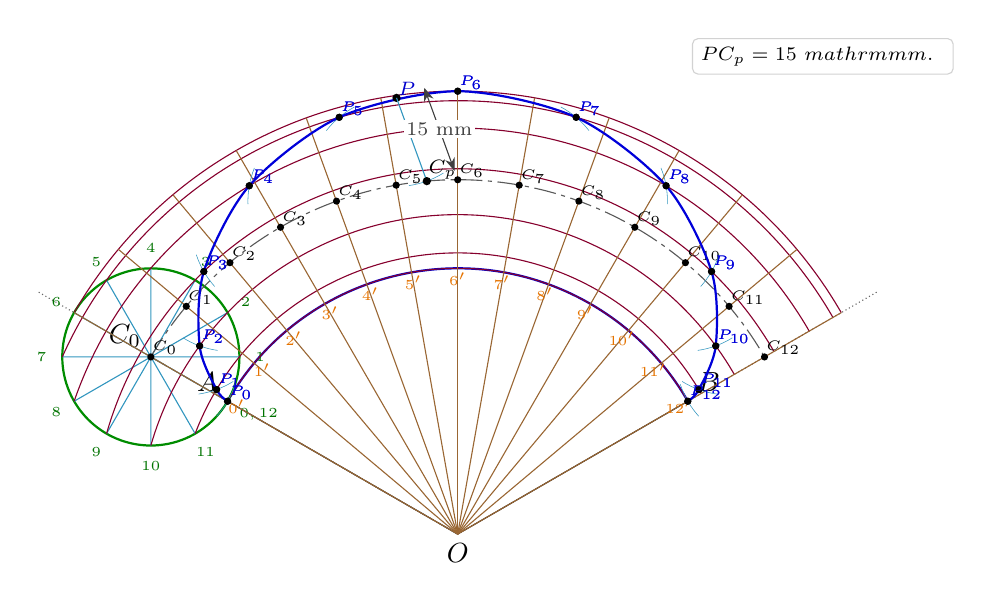
\begin{tikzpicture}[scale=.075,>=stealth]\FinalConstruction\SelectedGeometry\PGeometry\PtoCpArc\Legend{$PC_p=15\ mathrm{mm}$.}\end{tikzpicture}\end{frame}
\begin{frame}{Step 17: Join $C_p$ to $O$}\centering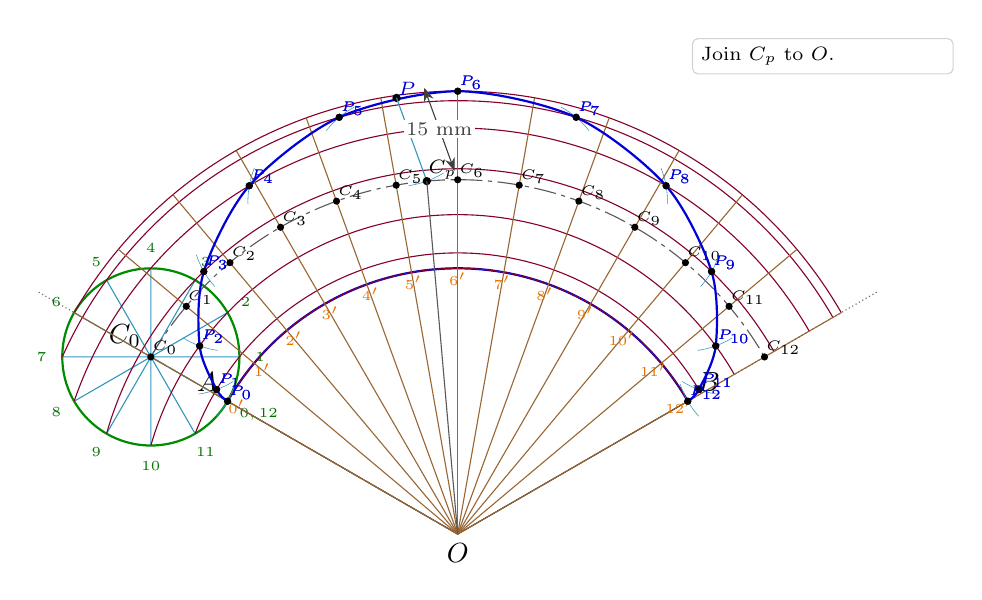
\begin{tikzpicture}[scale=.075,>=stealth]\FinalConstruction\SelectedGeometry\PGeometry\PtoCpArc\draw[contact line](O)--(Cp);\Legend{Join $C_p$ to $O$.}\end{tikzpicture}\end{frame}
\begin{frame}{Step 18: Mark $M$ on the directing circle}\centering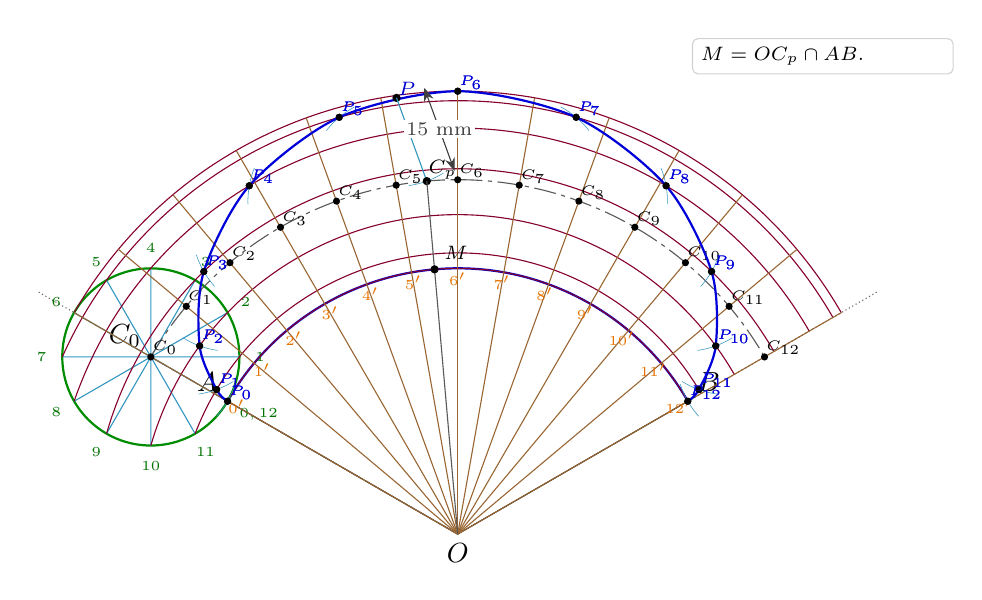
\begin{tikzpicture}[scale=.075,>=stealth]\FinalConstruction\SelectedGeometry\PGeometry\PtoCpArc\draw[contact line](O)--(Cp);\node[fill=black,circle,minimum size=3.0pt,inner sep=0pt,outer sep=0pt,transform shape=false]at(M){};\node[font=\scriptsize,above right]at(M){$M$};\Legend{$M=OC_p\cap AB$.}\end{tikzpicture}\end{frame}
\newcommand{\NormalLine}{
  \draw[normal line,line width=1.2pt](NNleft)--(NNright);
  \node[
    font=\scriptsize,
    orange!85!black,
    above right,
    xshift=2pt
  ] at (NNright) {$N'$};
  \node[
    font=\scriptsize,
    orange!85!black,
    below left,
    xshift=-2pt
  ] at (NNleft) {$N$};
}
\begin{frame}{Step 19: Draw the normal $NN'$ through $P$}
\centering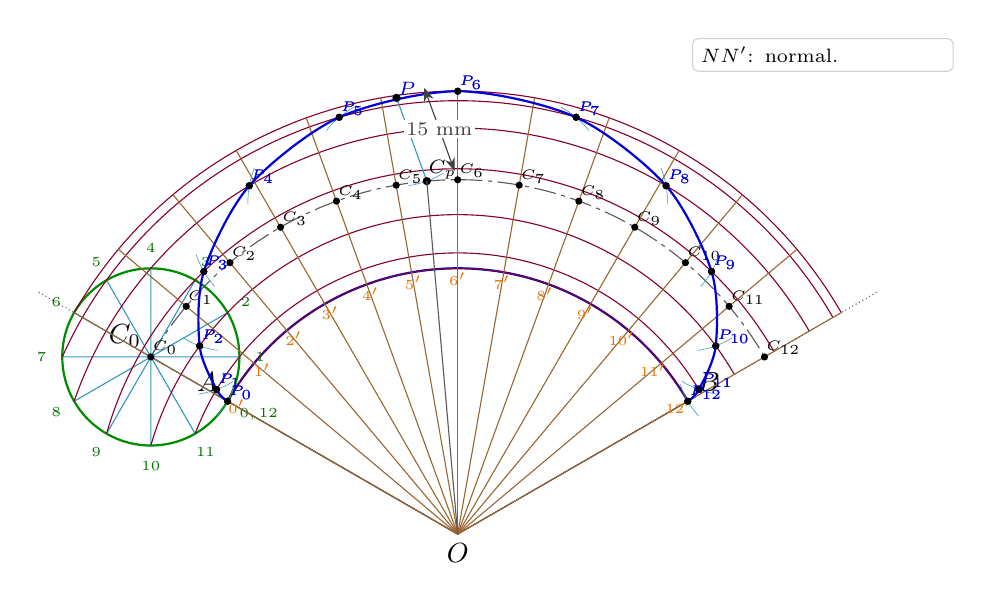
\begin{tikzpicture}[scale=.075,>=stealth]\FinalConstruction\SelectedGeometry\PtoCpArc\draw[contact line](O)--(Cp);\NormalLine\PGeometry\Legend{$NN'$: normal.}\end{tikzpicture}
\end{frame}
\begin{frame}{Step 20: Draw the tangent perpendicular to $NN'$}\centering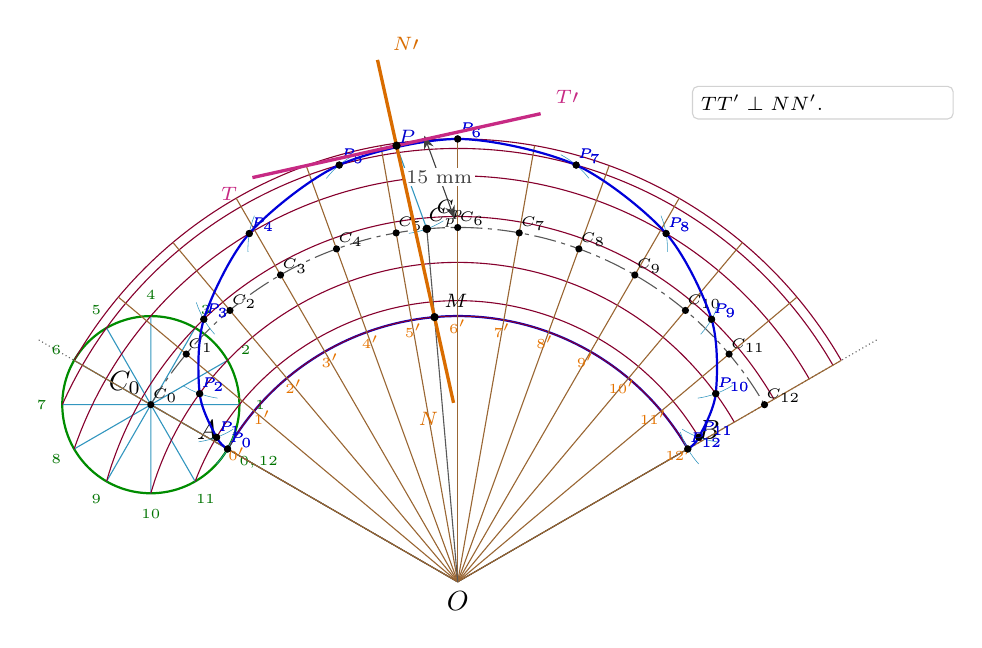
\begin{tikzpicture}[scale=.075,>=stealth]\FinalConstruction\SelectedGeometry\PtoCpArc\draw[contact line](O)--(Cp);\NormalAndTangent\PGeometry\node[fill=black,circle,minimum size=3.0pt,inner sep=0pt,outer sep=0pt,transform shape=false]at(M){};\node[font=\scriptsize,above right]at(M){$M$};\node[fill=black,circle,minimum size=3.0pt,inner sep=0pt,outer sep=0pt,transform shape=false]at(Cp){};\node[font=\scriptsize,above right]at(Cp){$C_p$};\Legend{$TT'\perp NN'$.}\end{tikzpicture}\end{frame}
\begin{frame}{Step 20: Show the right-angle at $P$}\centering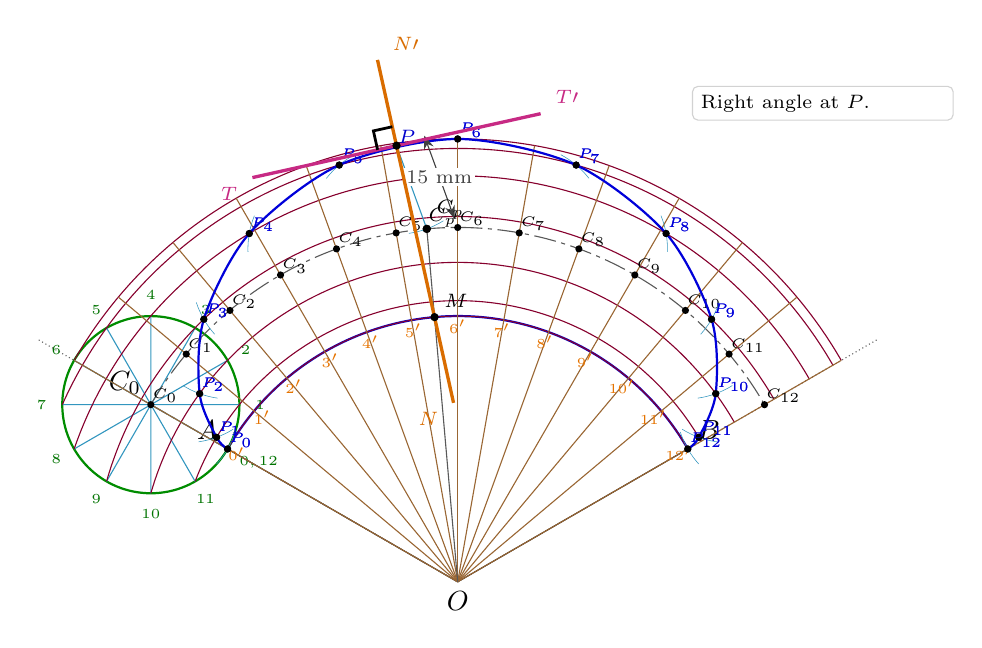
\begin{tikzpicture}[scale=.075,>=stealth]\FinalConstruction\SelectedGeometry\PtoCpArc\draw[contact line](O)--(Cp);\NormalAndTangent\PGeometry\node[fill=black,circle,minimum size=3.0pt,inner sep=0pt,outer sep=0pt,transform shape=false]at(M){};\node[font=\scriptsize,above right]at(M){$M$};\node[fill=black,circle,minimum size=3.0pt,inner sep=0pt,outer sep=0pt,transform shape=false]at(Cp){};\node[font=\scriptsize,above right]at(Cp){$C_p$};\pic[draw=black,line width=1pt,angle radius=7pt,angle eccentricity=1.35]at(Psel){right angle=T2--Psel--NNright};\Legend{Right angle at $P$.}\end{tikzpicture}\end{frame}
\begin{frame}{Step 20: Final completed epicycloid construction}\centering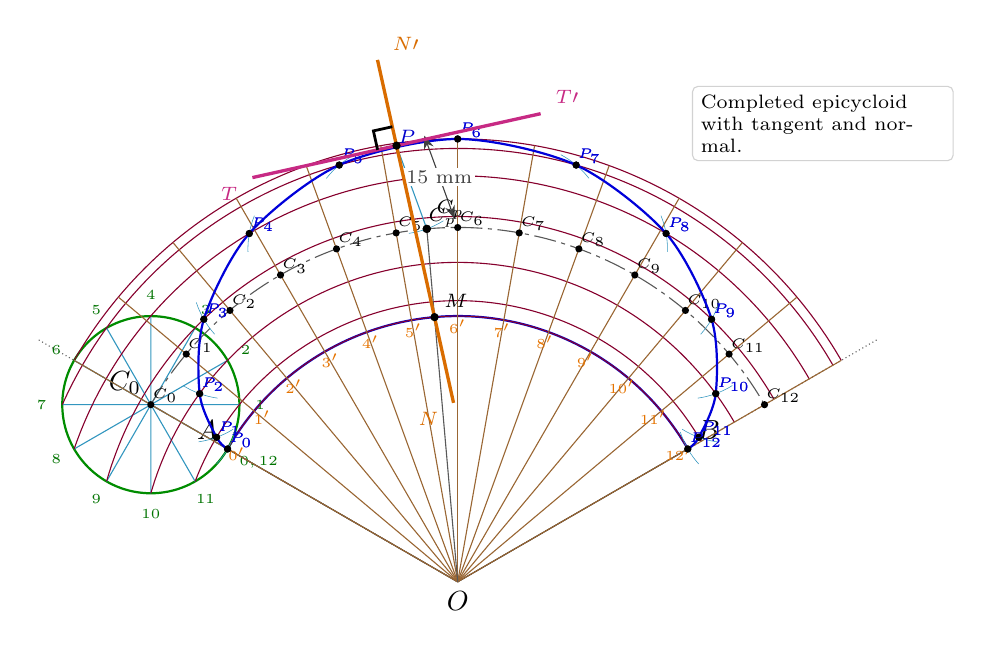
\begin{tikzpicture}[scale=.075,>=stealth]\FinalConstruction\SelectedGeometry\PtoCpArc\draw[contact line](O)--(Cp);\NormalAndTangent\PGeometry\node[fill=black,circle,minimum size=3.0pt,inner sep=0pt,outer sep=0pt,transform shape=false]at(M){};\node[font=\scriptsize,above right]at(M){$M$};\node[fill=black,circle,minimum size=3.0pt,inner sep=0pt,outer sep=0pt,transform shape=false]at(Cp){};\node[font=\scriptsize,above right]at(Cp){$C_p$};\pic[draw=black,line width=1pt,angle radius=7pt,angle eccentricity=1.35]at(Psel){right angle=T2--Psel--NNright};\Legend{Completed epicycloid with tangent and normal.}\end{tikzpicture}\end{frame}
\end{document}
